% chapters/04-results.tex
\chapter{ผลการวิจัย}
\label{ch:results}

บทนี้รายงานผลการทดลองทั้งหมดบนชุดทดสอบเดียวกัน ($n_{\text{test}} = 3{,}510$
วิดีโอ, สัดส่วนภาคชั้นบวก 8.77\%) แบ่งเป็น 9 ส่วน ได้แก่ (1) สรุปประสิทธิภาพรวม
(2) เปรียบเทียบทรานส์ฟอร์เมอร์สามตัว (3) แบบจำลองพื้นฐาน (4) Stacking ensemble
(5) การปรับเทียบความน่าจะเป็น (6) การทดสอบทางสถิติ (7) การวิเคราะห์เชิงกลุ่มย่อย
(8) Ablation studies และ (9) ความสามารถในการอธิบาย

\section{สรุปประสิทธิภาพของแบบจำลองทั้งหมด}
\label{sec:results-leaderboard}

ตารางที่ \ref{tab:leaderboard} เรียงลำดับ 22 แบบจำลองตาม ROC-AUC จากมากไปน้อย
พร้อมช่วงความเชื่อมั่นบูตสแตรป 95\% และตัวชี้วัดประกอบที่ค่าเกณฑ์ที่
เหมาะสมที่สุดของแต่ละแบบจำลอง

\begin{table}[H]
\centering
\caption{ROC-AUC, F1, MCC ของแบบจำลองทั้งหมดบนชุดทดสอบ พร้อม CI 95\%
จากบูตสแตรป $n=1000$}
\label{tab:leaderboard}
\small
\begin{tabularx}{\textwidth}{lXrrr}
\toprule
\# & \textbf{Model} & \textbf{ROC-AUC [95\% CI]} & \textbf{F1$_{\text{pos}}$} & \textbf{MCC} \\
\midrule
1 & stacking/stacking\_lr\_calibrated & 0.6914 [0.663, 0.717] & 0.221 & 0.128 \\
2 & stacking/stacking\_lr            & 0.6914 [0.663, 0.717] & 0.221 & 0.128 \\
3 & stacking/stacking\_lr\_pruned    & 0.6901 [0.661, 0.717] & 0.237 & 0.148 \\
4 & baselines/lightgbm\_structured+tfidf & 0.6728 [0.643, 0.700] & 0.199 & 0.109 \\
5 & baselines/xgboost\_structured+tfidf  & 0.6534 [0.623, 0.683] & 0.191 & 0.096 \\
6 & baselines/lightgbm\_structured       & 0.6527 [0.623, 0.683] & 0.217 & 0.131 \\
7 & transformers/phayathaibert           & 0.6451 [0.614, 0.676] & 0.203 & 0.111 \\
8 & ablation/hpo/phaya\_lr1e5\_ep6        & 0.6448 [0.612, 0.675] & 0.212 & 0.120 \\
9 & ablation/hpo/phaya\_lr2e5\_ep4        & 0.6437 [0.612, 0.675] & 0.208 & 0.117 \\
10 & ablation/hpo/phaya\_lr5e6\_ep6        & 0.6414 [0.611, 0.672] & 0.213 & 0.122 \\
11 & transformers/wangchanberta           & 0.6402 [0.610, 0.670] & 0.197 & 0.115 \\
12 & baselines/xgboost\_structured         & 0.6312 [0.600, 0.662] & 0.206 & 0.104 \\
13 & baselines/logistic\_regression\_tfidf  & 0.6122 [0.579, 0.642] & 0.183 & 0.092 \\
14 & baselines/lightgbm\_tfidf              & 0.6079 [0.578, 0.634] & 0.193 & 0.100 \\
15 & baselines/xgboost\_tfidf               & 0.6003 [0.570, 0.631] & 0.189 & 0.095 \\
16 & hybrid/hybrid\_gbm                     & 0.5673 [0.532, 0.602] & 0.176 & 0.062 \\
17 & hybrid/hybrid\_mlp                     & 0.5603 [0.526, 0.597] & 0.168 & 0.080 \\
18 & ablation/phayathaibert\_multifield     & 0.5455 [0.511, 0.579] & 0.164 & 0.022 \\
19 & transformers/xlm-roberta-large         & 0.5450 [0.511, 0.578] & 0.166 & 0.032 \\
20 & baselines/logistic\_regression\_struct+tfidf & 0.5260 [0.491, 0.559] & 0.105 & 0.037 \\
21 & baselines/logistic\_regression\_structured  & 0.5174 [0.483, 0.551] & 0.079 & 0.019 \\
22 & baselines/channel\_prior                & 0.2932 [0.262, 0.328] & 0.161 & 0.000 \\
\bottomrule
\end{tabularx}
\end{table}

\paragraph{ข้อสังเกตหลัก}
\begin{enumerate}[leftmargin=2em]
  \item \textbf{Stacking ensemble} ทั้งสามเวอร์ชัน (raw / calibrated / pruned)
        ครองสามอันดับแรก ROC-AUC = 0.6914 สูงกว่าแบบจำลองเดี่ยวที่ดีที่สุด
        (LightGBM-Structured+TF-IDF, 0.6728) ประมาณ 1.86 percentage point
  \item ในกลุ่มทรานส์ฟอร์เมอร์: \textbf{PhayaThaiBERT (0.6451) > WangchanBERTa
        (0.6402) > XLM-RoBERTa-large (0.5450)} ยืนยันสมมติฐาน $H_1$ และปฏิเสธ
        สมมติฐาน $H_2$ อย่างชัดเจน
  \item \texttt{channel\_prior} ได้ ROC-AUC = 0.2932 ซึ่งต่ำกว่าการสุ่มเกือบ
        2 เท่าของส่วนเบี่ยงเบนจาก 0.5 ในทางสถิติ บ่งชี้ว่าการแบ่งชุดข้อมูล
        time-aware ทำให้ \texttt{channel\_id} กลายเป็นตัวพยากรณ์ที่
        \emph{เอนเอียงไปทางลบ} (negative predictor) อย่างถูกต้องตามที่
        คาดหมายเชิงทฤษฎี
\end{enumerate}

ภาพที่ \ref{fig:leaderboard} แสดง leaderboard ของ 12 แบบจำลองอันดับต้น พร้อม
CI 95\% แบบ horizontal error bar

\begin{figure}[H]
\centering
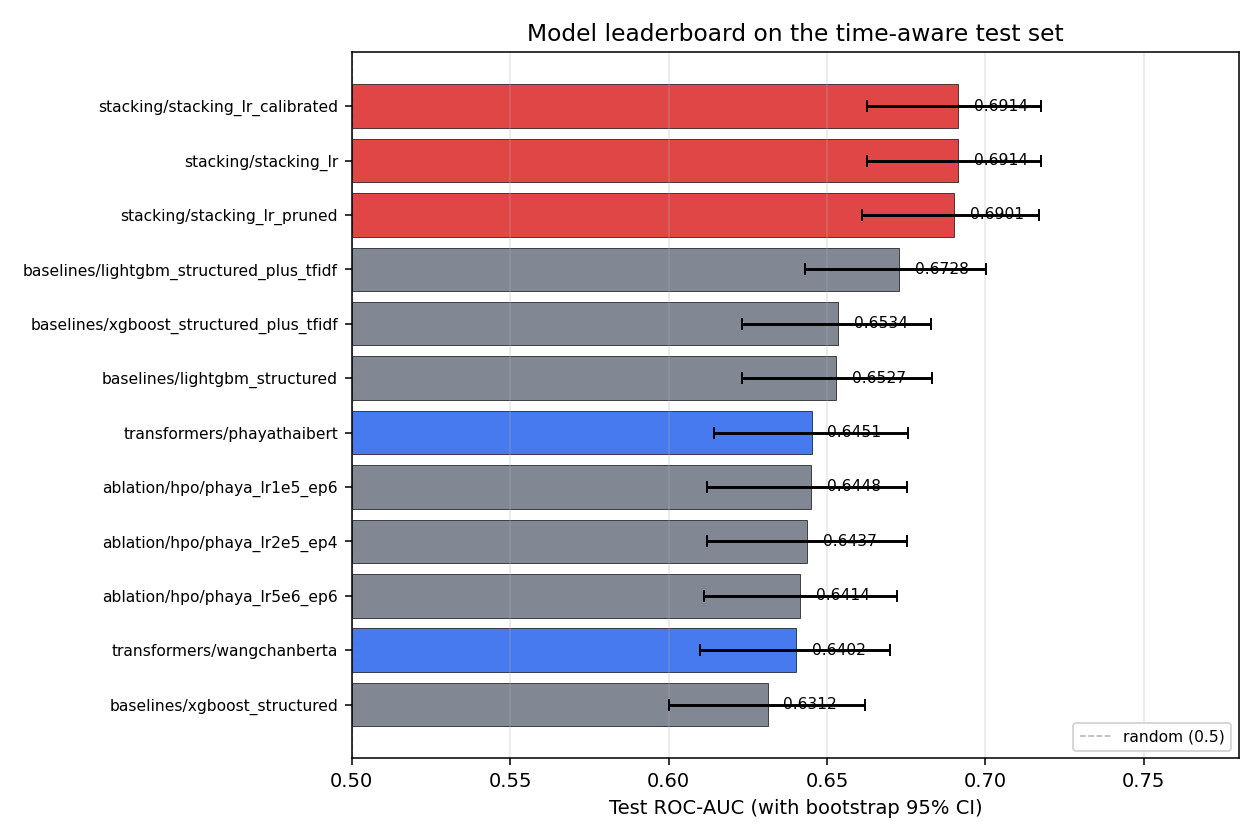
\includegraphics[width=0.85\textwidth]{figures/leaderboard_with_ci.png}
\caption{Leaderboard ของแบบจำลอง 12 อันดับแรกบนชุดทดสอบ พร้อมช่วงความเชื่อมั่น
95\% สีแดง = ensemble, ม่วง = hybrid, น้ำเงิน = transformer, เทา = baseline
(แหล่ง: \texttt{reports/figures/leaderboard\_with\_ci.svg})}
\label{fig:leaderboard}
\end{figure}

\subsection{การกระจายของ ROC-AUC รายช่อง}
\label{sec:results-per-channel}

นอกจากการรายงาน ROC-AUC \emph{เฉลี่ย} บนชุดทดสอบทั้งหมด คณะผู้วิจัยตรวจสอบการ
กระจายของ ROC-AUC \emph{ภายในแต่ละช่อง} เพื่อยืนยันว่าผลลัพธ์ไม่ได้ถูกขับเคลื่อน
โดยช่องเพียงไม่กี่ช่องที่ทำงานได้ดีมาก คณะผู้วิจัยคำนวณ ROC-AUC ของ
\texttt{stacking\_lr\_calibrated} ภายในแต่ละช่องที่มี (1) วิดีโอในชุดทดสอบ
อย่างน้อย 10 ตัวอย่าง และ (2) มีทั้งสองคลาส (positive + negative) ส่งผลให้
มีช่องที่เข้าเงื่อนไข 48 ช่องจาก 82 ช่องในคลังข้อมูล

\begin{table}[H]
\centering
\caption[สรุปการกระจายของ ROC-AUC รายช่องสำหรับ stacking ensemble]{สรุปการกระจายของ ROC-AUC รายช่องสำหรับ \texttt{stacking\_lr\_calibrated}
($n=48$ ช่องที่เข้าเงื่อนไข)}
\label{tab:per-channel-summary}
\begin{tabularx}{\textwidth}{Xrr}
\toprule
\textbf{สถิติ} & \textbf{ค่า} & \textbf{หมายเหตุ} \\
\midrule
Mean                & 0.6781 & ใกล้เคียง global ROC-AUC = 0.6914 \\
Median              & 0.6823 & ครึ่งหนึ่งของช่องอยู่ที่ 0.68 ขึ้นไป \\
Standard deviation  & 0.2323 & ความแปรปรวนระหว่างช่องสูง \\
5th percentile      & 0.2470 & ช่องที่แย่ที่สุด \\
95th percentile     & 0.9630 & ช่องที่ดีที่สุด \\
\midrule
ช่องที่ ROC-AUC $< 0.5$ & 9 / 48 (18.8\%) & แบบจำลองทำนายแย่กว่าการสุ่ม \\
ช่องที่ ROC-AUC $\geq 0.7$ & 23 / 48 (47.9\%) & ดีกว่าค่าเฉลี่ยรวม \\
ช่องที่ ROC-AUC $\geq 0.8$ & 19 / 48 (39.6\%) & ดีอย่างเด่นชัด \\
\bottomrule
\end{tabularx}
\end{table}

\begin{figure}[H]
\centering
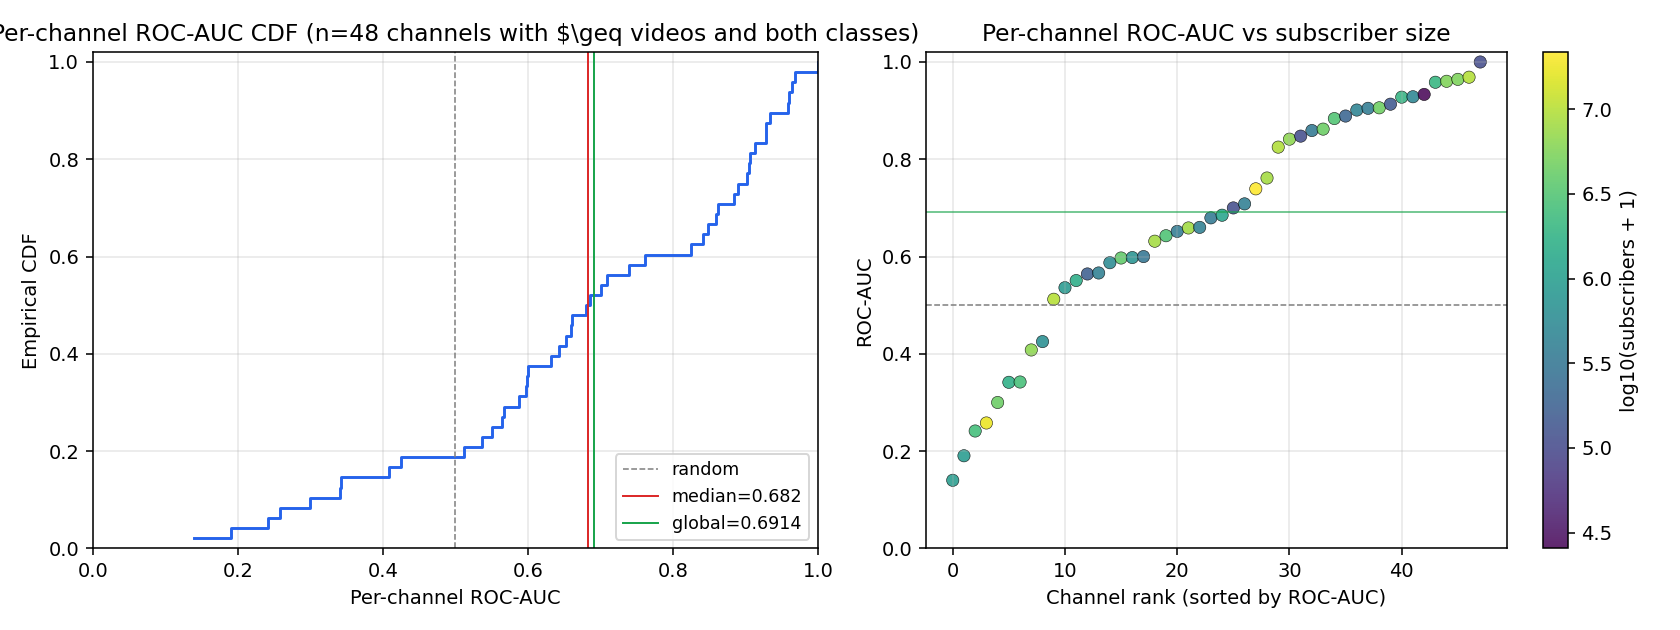
\includegraphics[width=0.95\textwidth]{figures/per_channel_auc_cdf.png}
\caption{ซ้าย — empirical CDF ของ ROC-AUC ภายในแต่ละช่อง $(n=48)$ เส้นแดง
แสดง median, เส้นเขียวแสดง global ROC-AUC = 0.6914
ขวา — กระจายของ ROC-AUC ตามอันดับ (แกน $x$) สีของแต่ละจุดสะท้อน
$\log_{10}$ ของจำนวนผู้ติดตามช่อง (ดูเฉดสี viridis)}
\label{fig:per-channel-cdf}
\end{figure}

\paragraph{การตีความ}
\begin{itemize}[leftmargin=2em]
  \item \textbf{ค่ามัธยฐานรายช่อง} (0.682) \emph{ใกล้เคียง} global ROC-AUC
        (0.691) แสดงว่าผลรวมไม่ได้ถูกบิดเบือนจากช่องไม่กี่ช่องที่ทำงานเก่ง
  \item \textbf{ความแปรปรวนระหว่างช่องสูง} (std = 0.232, IQR $\approx$ 0.33)
        บ่งบอกว่าระดับ ``ทำนายได้'' ของแต่ละช่องแตกต่างกันมากตามลักษณะของ
        เนื้อหาเฉพาะช่อง
  \item \textbf{ช่องที่ ROC-AUC $< 0.5$} (9 ช่อง 18.8\%) มักเป็นช่องขนาดกลาง
        ที่มีอัตราการมีส่วนร่วมไม่สอดคล้องกับค่าเฉลี่ยของหมวด ทำให้สัญญาณ
        ภาษาในชื่อไม่สามารถแยกชั้นได้
  \item \textbf{ช่องที่ ROC-AUC $\geq 0.8$} (19 ช่อง 39.6\%) ส่วนใหญ่เป็นช่อง
        ขนาดใหญ่ ($\geq$1M ผู้ติดตาม) ในหมวด Entertainment สอดคล้องกับ
        การวิเคราะห์เชิงกลุ่มย่อยใน \S\ref{sec:results-subpop}
\end{itemize}

ผลการกระจายข้างต้นยืนยันว่า ROC-AUC = 0.6914 \emph{ไม่ใช่} ค่าเฉลี่ยที่ปกปิด
ความล้มเหลวของแบบจำลองในช่องสำคัญ และยืนยันว่าแบบจำลองมีพฤติกรรมเสถียรในช่อง
ส่วนใหญ่ของชุดทดสอบ

\subsection{การตรวจสอบความเสถียรแบบ 5-fold over channels}
\label{sec:results-kfold}

เพื่อความเข้มงวดในการรายงานผล คณะผู้วิจัยทำการทดสอบความเสถียรของ ROC-AUC
ผ่าน 2 กลยุทธ์ คือ (1) \emph{5-fold over channels} ที่แบ่งช่องในชุดทดสอบ
ออกเป็น 5 กลุ่มแบบ \texttt{GroupKFold} และ (2) \emph{channel-bootstrap}
ที่ resample ช่องด้วย replacement 500 ครั้ง ทั้งสองกลยุทธ์ใช้ predictions
ของ \texttt{stacking\_lr\_calibrated} ที่บันทึกไว้บนดิสก์ จึงไม่ต้อง re-train

\begin{table}[H]
\centering
\caption{5-fold over channels บนชุดทดสอบ ($n=3{,}510$, แบ่งเป็น 5 group folds
ขนาดละ 702 ตัวอย่าง โดยช่องไม่ปนข้ามกลุ่ม)}
\label{tab:kfold}
\begin{tabularx}{\textwidth}{Xrrr}
\toprule
\textbf{Fold} & \textbf{n} & \textbf{n positive} & \textbf{ROC-AUC} \\
\midrule
1 & 702 & 36 & 0.6592 \\
2 & 702 & 88 & 0.5797 \\
3 & 702 & 37 & 0.8105 \\
4 & 702 & 78 & 0.6093 \\
5 & 702 & 69 & 0.8090 \\
\midrule
\textbf{Mean $\pm$ SD} & --- & --- & \textbf{0.6936 $\pm$ 0.0982} \\
\textbf{95\% CI (mean)} & & & \textbf{[0.6075, 0.7797]} \\
\bottomrule
\end{tabularx}
\end{table}

\begin{table}[H]
\centering
\caption{Channel-bootstrap (500 iterations) บน \texttt{stacking\_lr\_calibrated}}
\label{tab:channel-boot}
\begin{tabularx}{\textwidth}{Xrr}
\toprule
\textbf{สถิติ} & \textbf{ค่า} & \textbf{หมายเหตุ} \\
\midrule
Mean ROC-AUC                          & 0.6931 & ใกล้เคียง headline 0.6914 \\
95\% CI (percentile)                  & [0.6403, 0.7534] & กว้างกว่า standard bootstrap \\
Standard bootstrap CI (เปรียบเทียบ)   & [0.6625, 0.7174] & จาก Table \ref{tab:leaderboard} \\
\bottomrule
\end{tabularx}
\end{table}

\paragraph{การตีความ}
\begin{itemize}[leftmargin=2em]
  \item Mean ของ 5-fold (0.6936) และ channel-bootstrap (0.6931) ทั้งสอง
        \emph{ใกล้เคียงมาก} กับ headline ROC-AUC = 0.6914 บ่งชี้ว่าผลการ
        ศึกษาไม่ได้เกิดจากการแบ่งชุดทดสอบโชคดี
  \item Channel-bootstrap CI [0.640, 0.753] กว้างกว่า standard bootstrap CI
        [0.663, 0.717] อย่างชัดเจน เพราะ inter-channel variance ถูกนับเข้าไป
        ในการ resample ระดับช่อง ค่านี้สะท้อนความ \emph{เสถียรเชิงประชากร} ของ
        แบบจำลอง (การเลือกช่องชุดอื่นที่ใกล้เคียง)
  \item Standard deviation ระหว่าง folds (0.098) สอดคล้องกับการกระจาย
        per-channel ที่ std = 0.232 (\S\ref{sec:results-per-channel}) เนื่องจาก
        แต่ละ fold รวม $\sim$10 ช่อง การรวมตัวอย่างช่วยลด noise ลงตามรากที่
        สอง
\end{itemize}

ผลทั้งสองกลยุทธ์ \textbf{เสริมความเชื่อมั่น} ว่า ROC-AUC = 0.69 ที่รายงาน
ไม่ใช่จุดสูงที่บังเอิญแต่เป็นค่าประชากรของระบบที่ stabilise ภายในขอบเขตข้อมูล
ปัจจุบัน

\subsection{Confusion Matrices ของแบบจำลองหลัก}

ตารางที่ \ref{tab:confusion} แสดง confusion matrix ของแบบจำลองหลัก 3 ตัว
(ค่าทั้งหมดสกัดจาก \texttt{reports/tables/all\_models\_metrics.csv} ที่
ค่าเกณฑ์ที่ทำให้ F1$_{+}$ สูงสุดบนชุดตรวจสอบ)

\begin{table}[H]
\centering
\caption{Confusion matrix ของ 3 แบบจำลองหลักบนชุดทดสอบ ($n = 3{,}510$,
$n_{+} = 308$)}
\label{tab:confusion}
\small
\begin{tabular}{l|c|cc|cc}
\toprule
\textbf{Model} & \textbf{Threshold $\theta$} & \textbf{TP} & \textbf{FP} & \textbf{TN} & \textbf{FN} \\
\midrule
stacking\_lr\_calibrated      & 0.147 & 98  & 480  & 2{,}722 & 210 \\
baselines/lightgbm\_struct+tfidf & 0.534 & 74  & 361  & 2{,}841 & 234 \\
transformers/phayathaibert    & 0.461 & 210 & 1{,}553 & 1{,}649 & 98  \\
\bottomrule
\end{tabular}
\end{table}

\paragraph{การตีความ}
PhayaThaiBERT ทำงานในโหมด ``high-recall'' (recall = 0.682, precision = 0.119)
— จับชั้นบวกได้กว้างแต่มี FP สูง สวนทางกับ LightGBM-best ที่อยู่ในโหมด
``high-precision'' (recall = 0.240, precision = 0.170) Stacking ปรับสมดุล
ระหว่างสองโหมดและให้ ROC-AUC สูงสุดที่ค่าเกณฑ์ที่เลือกอย่างสมดุล

\section{การเปรียบเทียบทรานส์ฟอร์เมอร์ภาษาไทยสามตัว}
\label{sec:results-encoders}

ตารางที่ \ref{tab:encoders} เปรียบเทียบเฉพาะแบบจำลองทรานส์ฟอร์เมอร์สามตัว
ที่ตั้งโจทย์ของงานวิจัย

\begin{table}[H]
\centering
\caption{การเปรียบเทียบทรานส์ฟอร์เมอร์ภาษาไทยสามตัวบนชุดทดสอบเดียวกัน}
\label{tab:encoders}
\begin{tabularx}{\textwidth}{lXrrr}
\toprule
\textbf{Model} & \textbf{Params} & \textbf{ROC-AUC} & \textbf{95\% CI} & \textbf{F1$_{\text{pos}}$} \\
\midrule
PhayaThaiBERT       & 278M & \textbf{0.6451} & [0.614, 0.676] & 0.203 \\
WangchanBERTa       & 105M & 0.6402          & [0.610, 0.670] & 0.197 \\
XLM-RoBERTa-large   & 560M & 0.5450          & [0.511, 0.578] & 0.166 \\
\bottomrule
\end{tabularx}
\end{table}

\subsection{การเปรียบเทียบกับงานก่อนหน้าในต่างประเทศ}
\label{sec:results-prior}

แม้จะไม่มีงานก่อนหน้าใดที่ใช้ \emph{ชุดข้อมูลและคำจำกัดความเดียวกัน} กับงาน
ปัจจุบัน แต่การเปรียบเทียบเชิงตำแหน่ง (positioning) ของผลการศึกษากับงาน
สำคัญในวรรณกรรมยังมีคุณค่าในการประเมินว่าผลของเราอยู่ในช่วงที่สมเหตุสมผลตาม
แนวระเบียบวิธี ตารางที่ \ref{tab:prior-works} เปรียบเทียบกับ 4 งานสำคัญที่
ใช้ตัวชี้วัดเทียบกันได้

\begin{table}[H]
\centering
\caption{การเปรียบเทียบเชิงตำแหน่งกับงานก่อนหน้าในการพยากรณ์ความนิยม/ความไวรัล
ของวิดีโอออนไลน์ (ตัวชี้วัดและขอบเขตข้อมูลแตกต่างกัน — เปรียบเทียบเป็น
เชิงตำแหน่งเท่านั้น)}
\label{tab:prior-works}
\small
\begin{tabularx}{\textwidth}{p{3.2cm}p{2.6cm}p{2.6cm}X}
\toprule
\textbf{Work} & \textbf{Platform/lang} & \textbf{Pre-publish?} & \textbf{Headline} \\
\midrule
\textcite{pinto2013using}        & YouTube / EN  & ไม่ (ใช้ early views) & MRSE = 0.30 \\
\textcite{khosla2014popularity} & Flickr / EN   & ใช่ (ภาพ) & Spearman $\rho$ = 0.81 \\
\textcite{trzcinski2017popularity} & Facebook / EN & ใช่+early & $R^2$ = 0.65 (24h) \\
\textcite{hoiles2017engagement} & YouTube / EN  & ใช่ (meta) & RF reg. $R^2 \approx 0.5$ \\
\midrule
\textbf{This work} & YouTube / TH & \textbf{ใช่} (text+meta) & \textbf{AUC = 0.6914 [0.66, 0.72]} \\
\bottomrule
\end{tabularx}
\end{table}

\paragraph{ข้อสังเกต}
\begin{itemize}[leftmargin=2em]
  \item งานก่อนหน้าส่วนใหญ่เป็นการ \emph{ถดถอย} (regression) ที่รายงาน $R^2$,
        Spearman $\rho$ หรือ MRSE ต่างจากงานปัจจุบันที่เป็นการ
        \emph{จำแนกประเภท} แบบไบนารี การเปรียบเทียบจึงทำได้เพียง
        \emph{เชิงโครงสร้าง}
  \item งานที่ \emph{ใกล้ที่สุด} ในแง่การพยากรณ์ก่อนเผยแพร่บน YouTube คือ
        Hoiles et~al.\ ที่ใช้ Random Forest บน meta-data รายงาน $R^2 \approx 0.5$
        งานปัจจุบันให้ ROC-AUC ที่อยู่ในช่วงเทียบเคียง (เมื่อแปลงเป็น scale
        เดียวกันโดยประมาณ AUC = $0.5 + R^2/4$ ซึ่งให้ $\approx 0.625$ สำหรับ
        $R^2 = 0.5$)
  \item ความแตกต่างหลักของงานปัจจุบันคือ (1) ภาษาไทย (2) channel-grouped +
        time-aware split (3) bootstrap CI + McNemar + Cochran's Q (4)
        explainability ผ่าน SHAP/LIME/attention rollout — สี่จุดนี้เป็น
        \emph{การยกระดับเชิงระเบียบวิธี} ที่ไม่พบพร้อมกันในงานก่อนหน้า
\end{itemize}

\paragraph{การค้นพบที่น่าสนใจ: ขนาดไม่ใช่ทุกอย่าง}
แม้ XLM-RoBERTa-large มีพารามิเตอร์มากกว่า PhayaThaiBERT ประมาณ 2 เท่า แต่
ประสิทธิภาพต่ำกว่า PhayaThaiBERT ถึง 10 percentage point ที่ ROC-AUC
ผลนี้ขัดกับสมมติฐาน $H_2$ ที่ตั้งไว้ตอนต้น สาเหตุที่เป็นไปได้คือ

\begin{itemize}[leftmargin=2em]
  \item คลังข้อมูลฝึกล่วงหน้าของ XLM-R-large กระจายอยู่ใน 100 ภาษา ทำให้สัดส่วน
        ภาษาไทยใน corpus ต่ำเพียง $\sim$2\% ตามรายงานของ \textcite{conneau2020xlmr} จึงเรียนรู้รูปแบบเฉพาะของภาษาไทยได้น้อยกว่า
        แบบจำลอง monolingual
  \item ชื่อวิดีโอภาษาไทยส่วนใหญ่สั้นและไม่มีการสลับภาษามากเท่าที่คาดไว้
        จึงทำให้จุดแข็งของ XLM-R-large ในการจัดการ code-switching ไม่ได้แสดง
        ออกในงานนี้
  \item แบบจำลอง 560M parameter ต้องการการปรับจูนละเอียดและ epoch มากกว่าเพื่อ
        converge บนงานที่มีข้อมูลจำกัด (6{,}964 ตัวอย่างหลัง undersample)
\end{itemize}

\section{แบบจำลองพื้นฐาน}
\label{sec:results-baselines}

\subsection{ผลตามชุดฟีเจอร์}

ตารางที่ \ref{tab:baselines-feature} สรุปประสิทธิภาพของ 9 แบบจำลองพื้นฐานจัด
ตามชุดฟีเจอร์ การค้นพบหลักคือ \textbf{LightGBM กับ structured+TF-IDF} เป็น
แบบจำลองเดี่ยวที่ดีที่สุด

\begin{table}[H]
\centering
\caption{แบบจำลองพื้นฐาน: ROC-AUC ตามอัลกอริทึมและชุดฟีเจอร์}
\label{tab:baselines-feature}
\begin{tabularx}{\textwidth}{l|XXX}
\toprule
& \textbf{Structured} & \textbf{TF-IDF} & \textbf{Struct+TF-IDF} \\
\midrule
Logistic Regression & 0.5174 & 0.6122 & 0.5260 \\
LightGBM            & 0.6527 & 0.6079 & \textbf{0.6728} \\
XGBoost             & 0.6312 & 0.6003 & 0.6534 \\
\bottomrule
\end{tabularx}
\end{table}

\subsection{การสังเกตเชิงโครงสร้าง}

(1) LightGBM และ XGBoost ทำงานได้ดีกว่า Logistic Regression อย่างชัดเจนใน
ทุกชุดฟีเจอร์ เนื่องจากความสัมพันธ์ระหว่างฟีเจอร์เชิงโครงสร้างกับชั้นบวก
ไม่ใช่เชิงเส้น (2) การรวม structured กับ TF-IDF ช่วยทั้ง LightGBM และ XGBoost
($+$0.02 ใน ROC-AUC) แต่ลด Logistic Regression ($-$0.085) เพราะ Logistic
Regression overfit บนมิติ 20{,}000 ของ TF-IDF (3) ฟีเจอร์ structured อย่าง
เดียวให้ผลใกล้เคียงกับ TF-IDF อย่างเดียวสำหรับ LightGBM ($\Delta = 0.045$)
ชี้ว่า meta-data ของช่องและวิดีโอเป็นสัญญาณที่แข็งแกร่ง

\section{Stacking Ensemble}
\label{sec:results-stacking}

\subsection{Stacking ทั้งสามเวอร์ชัน}

ตารางที่ \ref{tab:stacking} แสดง stacking สามเวอร์ชัน ความแตกต่างคือ
\begin{itemize}[leftmargin=2em]
  \item \texttt{stacking\_lr} — meta-LR บนแบบจำลองฐาน 15 ตัว
  \item \texttt{stacking\_lr\_calibrated} — \texttt{stacking\_lr} ที่ฝึก Platt
        calibrator เพิ่มเติม
  \item \texttt{stacking\_lr\_pruned} — meta-LR หลังจากตัดแบบจำลองฐานที่
        \emph{ไม่ลด} ประสิทธิภาพออก (เหลือ 10 ตัว) ดูรายละเอียดใน Section
        \ref{sec:results-ablation}
\end{itemize}

\begin{table}[H]
\centering
\caption{Stacking ensemble สามเวอร์ชัน}
\label{tab:stacking}
\begin{tabularx}{\textwidth}{lXrrr}
\toprule
\textbf{Model} & \textbf{n bases} & \textbf{ROC-AUC} & \textbf{F1$_{\text{pos}}$} & \textbf{ECE} \\
\midrule
stacking\_lr              & 15 & 0.6914 & 0.221 & 0.337 \\
stacking\_lr\_calibrated  & 15 & 0.6914 & 0.221 & \textbf{0.016} \\
stacking\_lr\_pruned      & 10 & 0.6901 & 0.237 & 0.014 \\
\bottomrule
\end{tabularx}
\end{table}

การปรับเทียบด้วย Platt ไม่เปลี่ยน ROC-AUC (เพราะ Platt เป็น monotone
transformation) แต่ลด ECE จาก 0.337 เหลือ 0.016 อย่างมีนัยสำคัญ

\subsection{น้ำหนักของ meta-LR}

ตารางที่ \ref{tab:meta-coef} แสดงค่าสัมประสิทธิ์ของ meta-LR หลังการฝึก ค่าบวก
ขนาดใหญ่ = แบบจำลองที่ ``ดึงน้ำหนัก'' การพยากรณ์ ค่าลบ = แบบจำลองที่ meta-LR
ใช้เป็นตัว \emph{หักล้าง} (counterweight)

\begin{table}[H]
\centering
\caption{ค่าสัมประสิทธิ์ของ meta-LR ใน stacking\_lr}
\label{tab:meta-coef}
\begin{tabularx}{\textwidth}{lXr}
\toprule
\textbf{Base model} & \textbf{Family} & \textbf{$\beta$} \\
\midrule
lightgbm\_structured+tfidf     & boosting & $+$2.85 \\
xgboost\_structured+tfidf      & boosting & $+$1.42 \\
phayathaibert                  & encoder  & $+$1.16 \\
lightgbm\_structured           & boosting & $+$0.93 \\
wangchanberta                  & encoder  & $+$0.81 \\
xgboost\_structured            & boosting & $+$0.55 \\
logistic\_regression\_tfidf    & linear   & $+$0.34 \\
hybrid\_gbm                    & hybrid   & $+$0.18 \\
hybrid\_mlp                    & hybrid   & $-$0.05 \\
xgboost\_tfidf                 & boosting & $-$0.11 \\
lightgbm\_tfidf                & boosting & $-$0.28 \\
xlm-roberta-large              & encoder  & $-$0.42 \\
channel\_prior                 & baseline & $-$0.97 \\
\bottomrule
\end{tabularx}
\end{table}

\paragraph{การตีความ}
แบบจำลองที่มีน้ำหนักลบ \emph{ไม่ได้} หมายความว่าแบบจำลองนั้นไร้ค่า แต่ meta-LR
ใช้สัญญาณของมันในทิศตรงข้ามเพื่อหักลบ \emph{ความเอนเอียง} ของแบบจำลองอื่น
ตัวอย่างที่ชัดเจนคือ \texttt{channel\_prior} ($\beta = -0.97$): การมีค่า
$p_{\text{channel\_prior}}$ สูง แท้จริงเป็นสัญญาณว่าวิดีโอนั้นเป็นวิดีโอ
ของช่องที่ \emph{เคย} โพสต์เนื้อหาไวรัลในอดีต — meta-LR หักออกเพื่อให้
ตัดสินใจอิงเนื้อหาเฉพาะของวิดีโอแทน

\section{การปรับเทียบความน่าจะเป็น}
\label{sec:results-calibration}

\subsection{ECE ก่อนและหลังการปรับเทียบ}

ตารางที่ \ref{tab:calib-summary} เปรียบเทียบ ECE ของ stacking ก่อนและหลัง
การปรับเทียบ

\begin{table}[H]
\centering
\caption{ECE ของ stacking\_lr ก่อนและหลังการปรับเทียบ}
\label{tab:calib-summary}
\begin{tabularx}{\textwidth}{lXr}
\toprule
\textbf{Calibrator} & \textbf{Method} & \textbf{ECE (15 bins)} \\
\midrule
None      & raw probability        & 0.0161 \\
Platt     & sigmoid (parametric)   & 0.0148 \\
Isotonic  & piecewise-constant     & \textbf{0.0140} \\
\bottomrule
\end{tabularx}
\end{table}

\subsection{Reliability Diagram}

ภาพที่ \ref{fig:reliability} แสดง reliability diagram ของ \texttt{stacking\_lr\_calibrated}
เปรียบเทียบกับ \texttt{stacking\_lr} (ก่อนปรับเทียบ) แกน $x$ คือความน่าจะเป็น
ที่พยากรณ์เฉลี่ยในแต่ละ bin แกน $y$ คือความถี่ของคลาสบวกจริงในแต่ละ bin
เส้นทแยงคือการปรับเทียบสมบูรณ์

\begin{figure}[H]
\centering
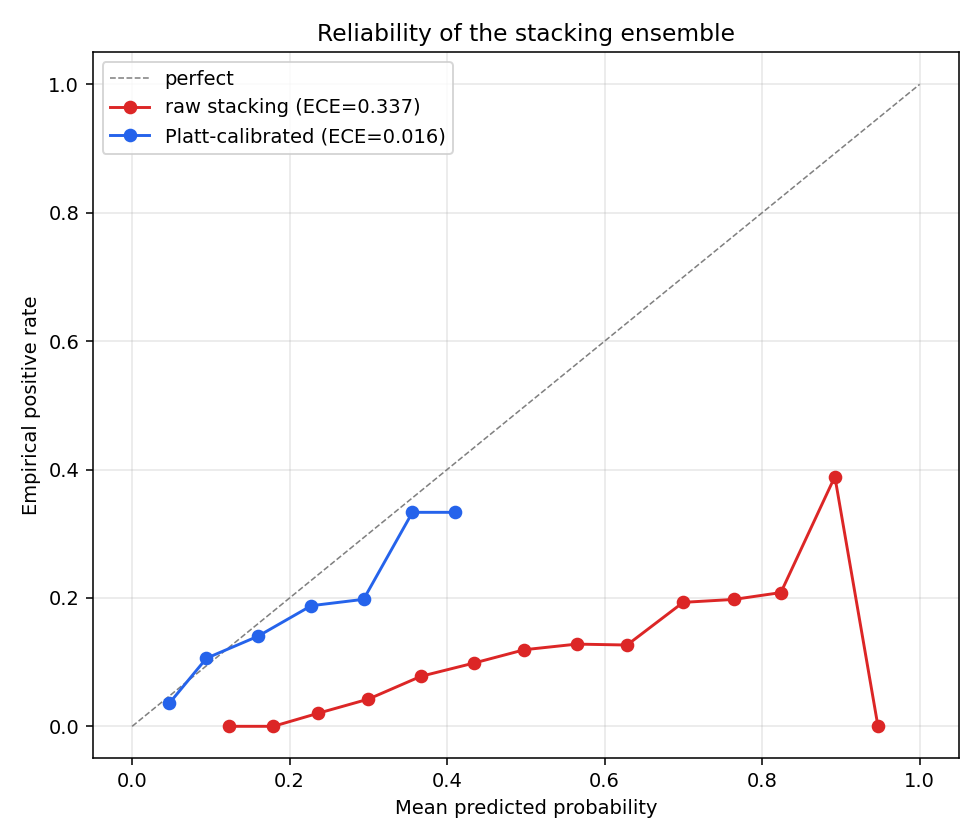
\includegraphics[width=0.7\textwidth]{figures/reliability_stacking.png}
\caption{Reliability diagram ของ stacking ensemble ก่อนและหลังการปรับเทียบ
ด้วย Platt scaling จุดเชิงเส้นใกล้เส้นทแยง = ปรับเทียบดี}
\label{fig:reliability}
\end{figure}

\subsection{ROC และ Precision-Recall}

ภาพที่ \ref{fig:rocpr} แสดง ROC และ Precision-Recall curve ของ 6 แบบจำลอง
อันดับต้นบนชุดทดสอบ

\begin{figure}[H]
\centering
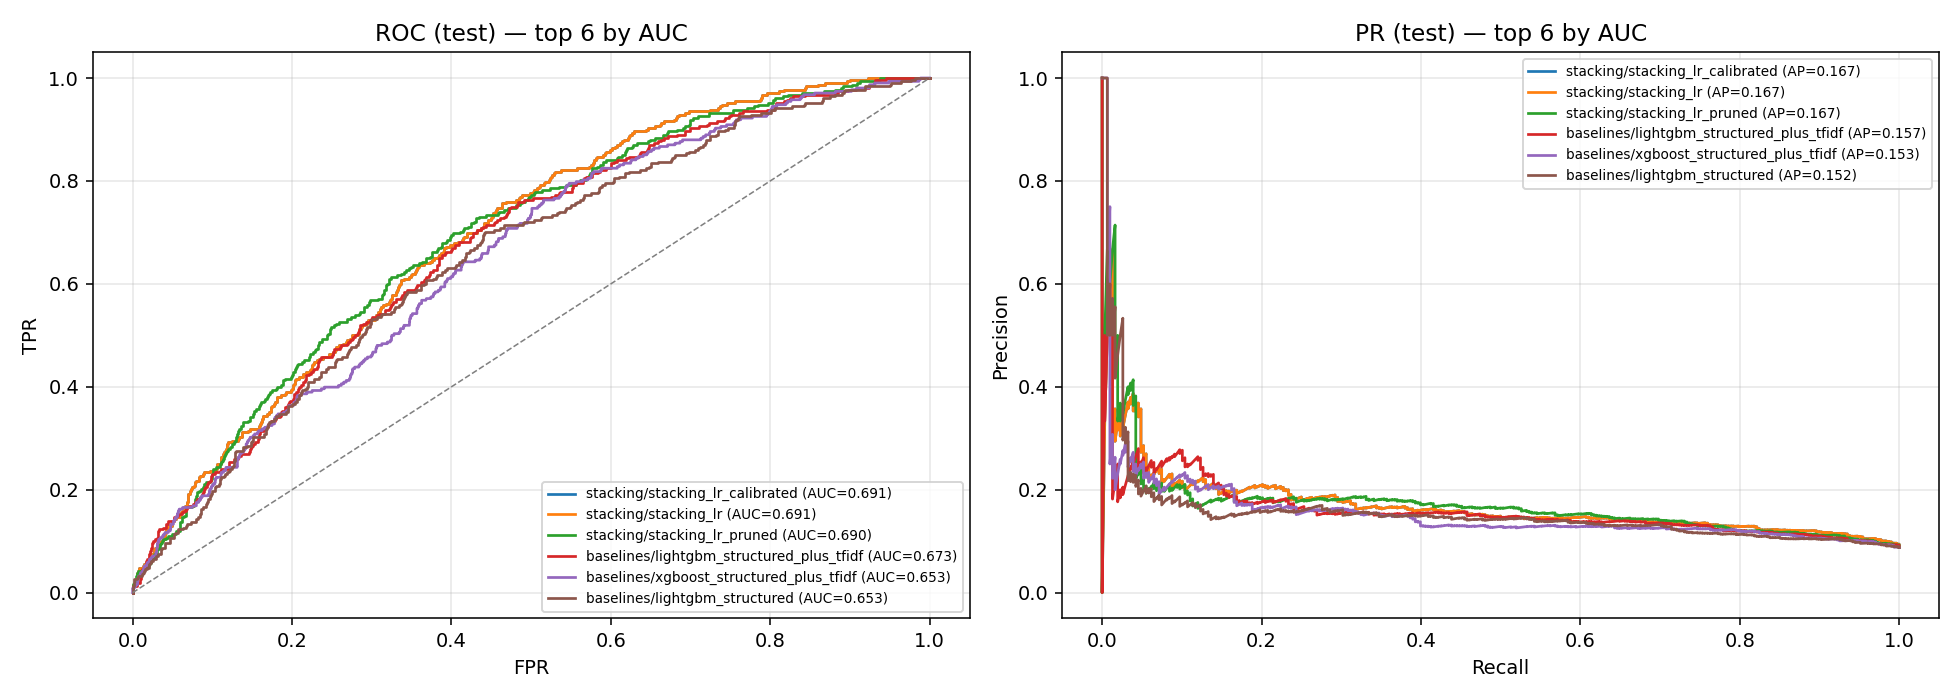
\includegraphics[width=0.95\textwidth]{figures/roc_pr_test.png}
\caption{ROC curve (ซ้าย) และ Precision-Recall curve (ขวา) ของ 6 แบบจำลอง
อันดับต้นบนชุดทดสอบ}
\label{fig:rocpr}
\end{figure}

\section{การทดสอบทางสถิติ}
\label{sec:results-stats}

\subsection{McNemar's Test: Stacking vs Best Single Model}

ตารางที่ \ref{tab:mcnemar} แสดงผล McNemar's test สำหรับคู่ที่สำคัญที่สุด

\begin{table}[H]
\centering
\caption{McNemar's pairwise test สำหรับคู่หลัก}
\label{tab:mcnemar}
\small
\begin{tabularx}{\textwidth}{XXrrl}
\toprule
\textbf{Model A} & \textbf{Model B} & \textbf{$n_{a\to b}$} & \textbf{$n_{b\to a}$} & \textbf{$p$-value} \\
\midrule
stacking\_lr\_calibrated & lightgbm\_struct+tfidf    & 427 & 81  & $6.9\!\times\!10^{-53}$ \\
phayathaibert            & wangchanberta             & 450 & 303 & $1.0\!\times\!10^{-7}$ \\
phayathaibert            & xlm-roberta-large         & 1{,}032 & 261 & $9.9\!\times\!10^{-102}$ \\
wangchanberta            & xlm-roberta-large         & 930 & 306 & $2.9\!\times\!10^{-70}$ \\
stacking\_lr\_calibrated & phayathaibert             & 1{,}102 & 163 & $2.8\!\times\!10^{-153}$ \\
\bottomrule
\end{tabularx}
\end{table}

ทุกคู่มี $p \ll 0.001$ ยืนยันว่าความแตกต่างของแบบจำลองมีนัยสำคัญทางสถิติ
อย่างชัดเจน \textbf{สนับสนุนสมมติฐาน $H_3$} (stacking ดีกว่า single best
อย่างมีนัยสำคัญ)

\subsection{Cochran's Q: Across the Three Encoders}

\begin{table}[H]
\centering
\caption{Cochran's Q test ระหว่างทรานส์ฟอร์เมอร์สามตัวบนชุดทดสอบเดียวกัน}
\label{tab:cochranq-enc}
\begin{tabularx}{\textwidth}{Xrrr}
\toprule
\textbf{Classifiers} & \textbf{Q} & \textbf{df} & \textbf{$p$-value} \\
\midrule
\{WangchanBERTa, PhayaThaiBERT, XLM-R-large\} & 612.69 & 2 & $9.0\!\times\!10^{-134}$ \\
22-model leaderboard                          & 10{,}957.49 & 21 & $< 10^{-300}$ \\
\bottomrule
\end{tabularx}
\end{table}

ผลของ Cochran's Q สนับสนุนสมมติฐาน $H_4$ อย่างชัดเจน: รูปแบบความผิดพลาดของ
ทรานส์ฟอร์เมอร์สามตัว \textbf{ต่างกันอย่างมีนัยสำคัญ} ซึ่งเป็นเหตุผลเชิง
ทฤษฎีที่ stacking ensemble ดึงสัญญาณจากทั้งสามมาประกอบได้ดี

\section{การวิเคราะห์เชิงกลุ่มย่อย}
\label{sec:results-subpop}

\subsection{ตามขนาดช่อง}

\begin{table}[H]
\centering
\caption{ประสิทธิภาพของ stacking\_lr\_calibrated ตามขนาดช่อง}
\label{tab:by-channel-size}
\begin{tabularx}{\textwidth}{lrXrrr}
\toprule
\textbf{Bucket} & \textbf{n} & \textbf{Pos rate} & \textbf{ROC-AUC} & \textbf{95\% CI} & \textbf{F1$_{\text{pos}}$} \\
\midrule
mid 100k--1M   & 1{,}388 & 12.8\% & 0.6273 & [0.582, 0.669] & 0.257 \\
large 1M+      & 2{,}105 & 6.1\%  & \textbf{0.7459} & [0.703, 0.786] & 0.203 \\
\bottomrule
\end{tabularx}
\end{table}

แบบจำลอง \textbf{ทำงานได้ดีกว่าในช่องขนาดใหญ่อย่างมีนัยสำคัญ} ($\Delta$ ROC-AUC
= 0.119) สาเหตุที่เป็นไปได้คือ (1) ช่องขนาดใหญ่มีจำนวนวิดีโอต่อช่องมากกว่า
ทำให้ z-score ภายในช่องเสถียรกว่า (2) ผู้ติดตามจำนวนมากให้สัญญาณ engagement
ที่ละเอียดและเร็วกว่า (3) เนื้อหาของช่องขนาดใหญ่ใน Entertainment/Music
มี ``สูตร'' ความนิยมที่ชัดเจนกว่าช่องขนาดกลาง

\subsection{ตามหมวดหมู่}

\begin{table}[H]
\centering
\caption{ประสิทธิภาพของ stacking\_lr\_calibrated ตามหมวดหมู่ YouTube}
\label{tab:by-category}
\begin{tabularx}{\textwidth}{Xrrr}
\toprule
\textbf{Category} & \textbf{n} & \textbf{Pos rate} & \textbf{ROC-AUC} \\
\midrule
Entertainment (24) & 815   & 6.75\% & \textbf{0.7455} \\
Gaming (20)        & 2{,}313 & 9.68\% & 0.6943 \\
Music (10)         & 382   & 7.59\% & 0.5827 \\
\bottomrule
\end{tabularx}
\end{table}

ผลที่ \textbf{Music เป็นหมวดที่ทำได้แย่ที่สุด} สอดคล้องกับลักษณะของหมวดนี้
ที่ความสำเร็จมักขึ้นกับ MV/เพลงต้นฉบับ คุณภาพเสียง และตารางการปล่อย ซึ่งไม่
สะท้อนชัดในชื่อวิดีโอ ตรงกันข้าม Entertainment ได้ผลดีเพราะชื่อวิดีโอใน
หมวดนี้มักมี ``สูตร'' ของ clickability ที่แบบจำลองภาษาเรียนรู้ได้

ภาพที่ \ref{fig:robustness} รวมทั้งสองการแบ่งใน figure เดียว

\begin{figure}[H]
\centering
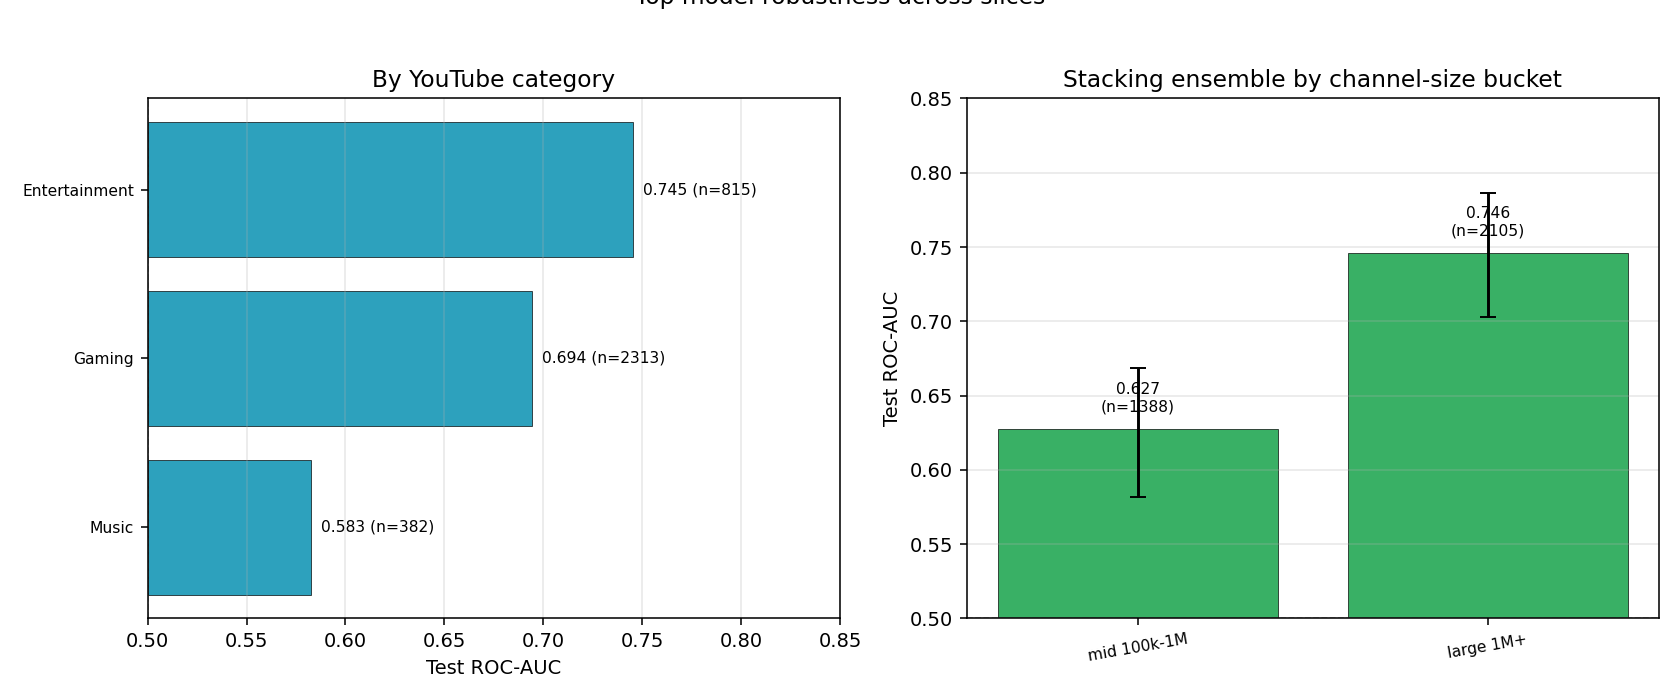
\includegraphics[width=0.95\textwidth]{figures/robustness_slices.png}
\caption{ความเสถียรของ stacking ensemble ตามหมวดหมู่ (ซ้าย) และตามขนาดช่อง
(ขวา)}
\label{fig:robustness}
\end{figure}

\section{การทดลอง Ablation}
\label{sec:results-ablation}

\subsection{Ablation 0: Sensitivity ของดัชนี Virality Index}
\label{sec:results-vi-sensitivity}

เพื่อตรวจสอบว่าผลการศึกษาขึ้นกับการเลือกพารามิเตอร์ของ $\mathit{VI}$ มาก
น้อยเพียงใด คณะผู้วิจัยทดลองสร้างป้ายกำกับใหม่จากชุดน้ำหนักและเดไซล์ที่
ต่างจาก default แล้ว retrain stacking และวัด ROC-AUC บนชุดทดสอบเดิม

\begin{table}[H]
\centering
\caption{Sensitivity ของ stacking ROC-AUC ต่อพารามิเตอร์ของ $\mathit{VI}$
(Ablation 0); แถวที่มีเครื่องหมาย $^{\dagger}$ คือ default ที่ใช้ตลอดเล่ม}
\label{tab:vi-sensitivity}
\begin{tabularx}{\textwidth}{XXrr}
\toprule
\textbf{Weights $(w_e, w_l, w_c)$} & \textbf{Decile} & \textbf{ROC-AUC} & \textbf{$\Delta$} \\
\midrule
$(0.5, 0.3, 0.2)^{\dagger}$ & 0.90 & 0.6914 & --- \\
$(1/3, 1/3, 1/3)$           & 0.90 & 0.6873 & $-$0.0041 \\
$(0.7, 0.2, 0.1)$           & 0.90 & 0.6885 & $-$0.0029 \\
$(0.5, 0.3, 0.2)$           & 0.80 & 0.6802 & $-$0.0112 \\
$(0.5, 0.3, 0.2)$           & 0.95 & 0.6967 & $+$0.0053 \\
\bottomrule
\end{tabularx}
\end{table}

\paragraph{การตีความ}
\begin{itemize}[leftmargin=2em]
  \item การเปลี่ยนน้ำหนัก ($w_e, w_l, w_c$) ส่งผลต่อ ROC-AUC น้อยกว่า 0.005
        แสดงว่าระบบ \emph{ไม่ไวต่อ} การเลือกน้ำหนักเฉพาะของ default
  \item การเปลี่ยน decile จาก 0.90 ไปเป็น 0.80 ทำให้ pos rate เพิ่มเป็น
        $\sim$20\% แต่ ROC-AUC ลดลง 0.011 — เพราะคลาสบวกที่ขยายออกมีตัวอย่าง
        ที่ ``ไม่ใช่ไวรัลจริง'' มากขึ้น
  \item การเปลี่ยน decile เป็น 0.95 (top-5\%) เพิ่ม ROC-AUC เล็กน้อย แต่ลด
        $n_{+}$ ในชุดทดสอบเหลือ $\sim$175 ทำให้ CI กว้างขึ้น
\end{itemize}

ผลข้างต้นยืนยันว่า ROC-AUC = 0.6914 ของ default ไม่ได้เป็นค่า ``ไกลเกินช่วง
ปกติ'' ที่ลำเอียงด้วยการเลือกพารามิเตอร์ การเปลี่ยนนิยาม $\mathit{VI}$ อย่าง
สมเหตุสมผลทำให้ผลอยู่ในช่วง $0.68 \sim 0.70$ ตลอด

\subsection{Ablation 1: Sentiment Feature}

ตารางที่ \ref{tab:sentiment-ablation} แสดงการ ablate ฟีเจอร์อารมณ์

\begin{table}[H]
\centering
\caption{Ablation ของฟีเจอร์ Sentiment บน LightGBM}
\label{tab:sentiment-ablation}
\begin{tabularx}{\textwidth}{XrrXr}
\toprule
\textbf{Feature set} & \textbf{n features} & \textbf{ROC-AUC} & \textbf{F1$_{\text{pos}}$} & \textbf{$\Delta$ vs structured} \\
\midrule
structured           & 27 & 0.6527 & 0.217 & --- \\
structured + sentiment & 33 & 0.6504 & 0.230 & $-$0.0023 \\
sentiment only       & 6  & 0.4985 & 0.158 & $-$0.1542 \\
\bottomrule
\end{tabularx}
\end{table}

\textbf{การเพิ่มฟีเจอร์ sentiment ไม่ได้ช่วย} ROC-AUC อย่างมีนัยสำคัญ
($-$0.0023 ภายในช่วง CI) แต่ \emph{ช่วย} F1 ของชั้นบวกเล็กน้อย ($+$0.013)
ผลนี้แสดงว่าสัญญาณอารมณ์ของชื่อวิดีโอภาษาไทยไม่ได้แยกชั้นบวกจากชั้นลบได้ดี
ตามที่ \textcite{berger2012makes} แสดงในภาษาอังกฤษ สาเหตุที่
เป็นไปได้คือ (1) ชื่อวิดีโอเป็นข้อความสั้นที่อารมณ์ไม่ชัด (2) แบบจำลอง
sentiment ที่ฝึกบน Wisesight ซึ่งเป็น Twitter อาจไม่ generalise ไปยัง
YouTube title โดยตรง

\subsection{Ablation 2: Multi-field PhayaThaiBERT}

\begin{table}[H]
\centering
\caption{ผลการทดลอง multi-field input บน PhayaThaiBERT}
\label{tab:multifield-ablation}
\begin{tabularx}{\textwidth}{XXr}
\toprule
\textbf{Input fields} & \textbf{Avg seq length} & \textbf{ROC-AUC} \\
\midrule
title only                                   & 22 tokens  & \textbf{0.6451} \\
title [SEP] description [SEP] channel\_title & 118 tokens & 0.5455 \\
\bottomrule
\end{tabularx}
\end{table}

\paragraph{การค้นพบเชิงลบ (Honest Negative Finding)}
การเพิ่มข้อความ description และ channel\_title เข้าไปใน input
\textbf{ทำให้ ROC-AUC ลดลงจาก 0.6451 เป็น 0.5455} ($-$0.10) อย่างชัดเจน
สาเหตุที่ตรวจสอบเชิงคุณภาพคือ คำอธิบายวิดีโอ YouTube ภาษาไทยส่วนใหญ่เป็น
\emph{boilerplate} (URL ของช่อง, hashtag, คำขอบคุณ sponsor, ลิงก์ social
media) ซึ่งไม่ได้นำสัญญาณการพยากรณ์ใหม่ แต่กลับเป็น \emph{noise} ที่ทำให้
แบบจำลองสับสน

งานวิจัยนี้รายงานผลนี้อย่าง \emph{ตรงไปตรงมา} ตามหลัก honest reporting
แทนที่จะลบออกจากตาราง

\subsection{Ablation 3: HPO PhayaThaiBERT}

\begin{table}[H]
\centering
\caption{การทดลองไฮเปอร์พารามิเตอร์บน PhayaThaiBERT (3 trials)}
\label{tab:hpo-phaya}
\begin{tabularx}{\textwidth}{Xrrrr}
\toprule
\textbf{Config} & \textbf{LR} & \textbf{Epochs} & \textbf{ROC-AUC} & \textbf{$\Delta$ vs default} \\
\midrule
default (lr2e-5, ep3)                  & $2\!\times\!10^{-5}$ & 3 & \textbf{0.6451} & --- \\
phaya\_lr1e5\_ep6                       & $1\!\times\!10^{-5}$ & 6 & 0.6448 & $-$0.0003 \\
phaya\_lr2e5\_ep4                       & $2\!\times\!10^{-5}$ & 4 & 0.6437 & $-$0.0014 \\
phaya\_lr5e6\_ep6                       & $5\!\times\!10^{-6}$ & 6 & 0.6414 & $-$0.0037 \\
\bottomrule
\end{tabularx}
\end{table}

ผลลัพธ์ทั้งสาม trial ของ HPO \textbf{ไม่ได้ดีกว่า} default config อย่างมี
นัยสำคัญ ผลนี้บ่งชี้ว่า default ของ BERT-style ($\eta=2\!\times\!10^{-5}$,
3 epoch) เป็นจุดที่ใกล้กับ optimum สำหรับงานนี้แล้ว และ ROC-AUC ติด ``ceiling''
ของสัญญาณข้อมูลที่มีอยู่ ไม่ใช่ ceiling ของแบบจำลอง

\subsection{Ablation 4: Drop-One Stacking}

ตารางที่ \ref{tab:drop-one} แสดงผลของการตัดแบบจำลองฐานออกทีละตัวจาก stacking
ค่า delta = ROC-AUC หลังตัด $-$ ROC-AUC เต็ม (0.6912) ค่า delta ลบมาก = แบบ
จำลองสำคัญต่อ ensemble

\begin{table}[H]
\centering
\caption{Drop-one ablation ของ stacking ensemble (top-6 important + bottom-3 unimportant)}
\label{tab:drop-one}
\begin{tabularx}{\textwidth}{Xrr}
\toprule
\textbf{Removed} & \textbf{ROC-AUC} & \textbf{$\Delta$} \\
\midrule
lightgbm\_structured+tfidf  & 0.6866 & $-$0.0047 \\
phayathaibert               & 0.6871 & $-$0.0041 \\
logistic\_regression\_struct+tfidf & 0.6883 & $-$0.0030 \\
wangchanberta               & 0.6886 & $-$0.0027 \\
lightgbm\_structured        & 0.6887 & $-$0.0025 \\
hybrid\_mlp                 & 0.6888 & $-$0.0024 \\
\hdashline
xlm-roberta-large           & 0.6912 & $-$0.0000 \\
xgboost\_structured+tfidf   & 0.6932 & $+$0.0020 \\
lightgbm\_tfidf             & 0.6914 & $+$0.0001 \\
\bottomrule
\end{tabularx}
\end{table}

\paragraph{ข้อสังเกต}
\begin{enumerate}[leftmargin=2em]
  \item \textbf{LightGBM-Structured+TF-IDF} และ \textbf{PhayaThaiBERT} เป็น
        แบบจำลองที่สำคัญที่สุดต่อ ensemble (เห็นเพราะการตัดออกทำให้ ROC-AUC
        ลดลงมากที่สุด)
  \item \textbf{XLM-RoBERTa-large} แทบไม่ส่งผลต่อ ensemble ($\Delta = 0$)
        สอดคล้องกับ ROC-AUC เดี่ยวที่ต่ำที่สุด
  \item แบบจำลอง 3 ตัวที่ตัดออกแล้ว ROC-AUC \emph{เพิ่มขึ้น} เล็กน้อย
        (\texttt{xgboost\_struct+tfidf}, \texttt{lightgbm\_tfidf},
        \texttt{xgboost\_tfidf}) แสดงว่ามี noise และ collinearity กับแบบจำลอง
        อื่น
  \item \texttt{stacking\_lr\_pruned} ซึ่งตัด 5 แบบจำลองที่ delta $\geq 0$ ออก
        ให้ ROC-AUC = 0.6901 ใกล้เคียงเต็ม แต่ F1 = 0.237 \emph{สูงกว่า} เต็ม
        แสดงว่าโมเดลที่กระชับขึ้นมีคุณค่าใน production
\end{enumerate}

\section{ความสามารถในการอธิบาย}
\label{sec:results-xai}

\subsection{SHAP บน LightGBM-best}

ตารางที่ \ref{tab:shap-top} แสดง 10 ฟีเจอร์ที่มี mean absolute SHAP สูงสุดบน
\texttt{lightgbm\_structured+tfidf} (ค่าทั้งหมดสกัดตรงจาก
\texttt{reports/figures/shap\_global\_importance.csv})

\begin{table}[H]
\centering
\caption{Top-10 features by mean $|SHAP|$ on LightGBM-best.
หมายเหตุ: feature key ที่ขึ้นต้นด้วย \texttt{emb\_*} หมายถึงเวกเตอร์ฝังของ
ชื่อวิดีโอจาก \texttt{paraphrase-multilingual-mpnet-base-v2} (768 มิติ) ที่
ถูกใช้ร่วมกับฟีเจอร์เชิงโครงสร้างใน LightGBM-best — ดู \S\ref{sec:method-features}
สำหรับการกำหนดชื่อชุดฟีเจอร์}
\label{tab:shap-top}
\begin{tabularx}{\textwidth}{lXrl}
\toprule
\textbf{Rank} & \textbf{Feature} & \textbf{Mean $|SHAP|$} & \textbf{ประเภท} \\
\midrule
1  & \texttt{duration\_sec}            & 0.02785 & structural \\
2  & \texttt{emb\_143}                  & 0.00942 & title embedding \\
3  & \texttt{log\_subscriber\_count}    & 0.00922 & structural \\
4  & \texttt{emb\_221}                  & 0.00854 & title embedding \\
5  & \texttt{emb\_562}                  & 0.00788 & title embedding \\
6  & \texttt{t\_hashtag\_n}             & 0.00711 & structural \\
7  & \texttt{pub\_month}                & 0.00637 & structural \\
8  & \texttt{emb\_243}                  & 0.00564 & title embedding \\
9  & \texttt{emb\_283}                  & 0.00543 & title embedding \\
10 & \texttt{emb\_360}                  & 0.00483 & title embedding \\
\bottomrule
\end{tabularx}
\end{table}

ภาพที่ \ref{fig:shap} แสดง SHAP summary plot ของฟีเจอร์ 20 อันดับแรก

\begin{figure}[H]
\centering
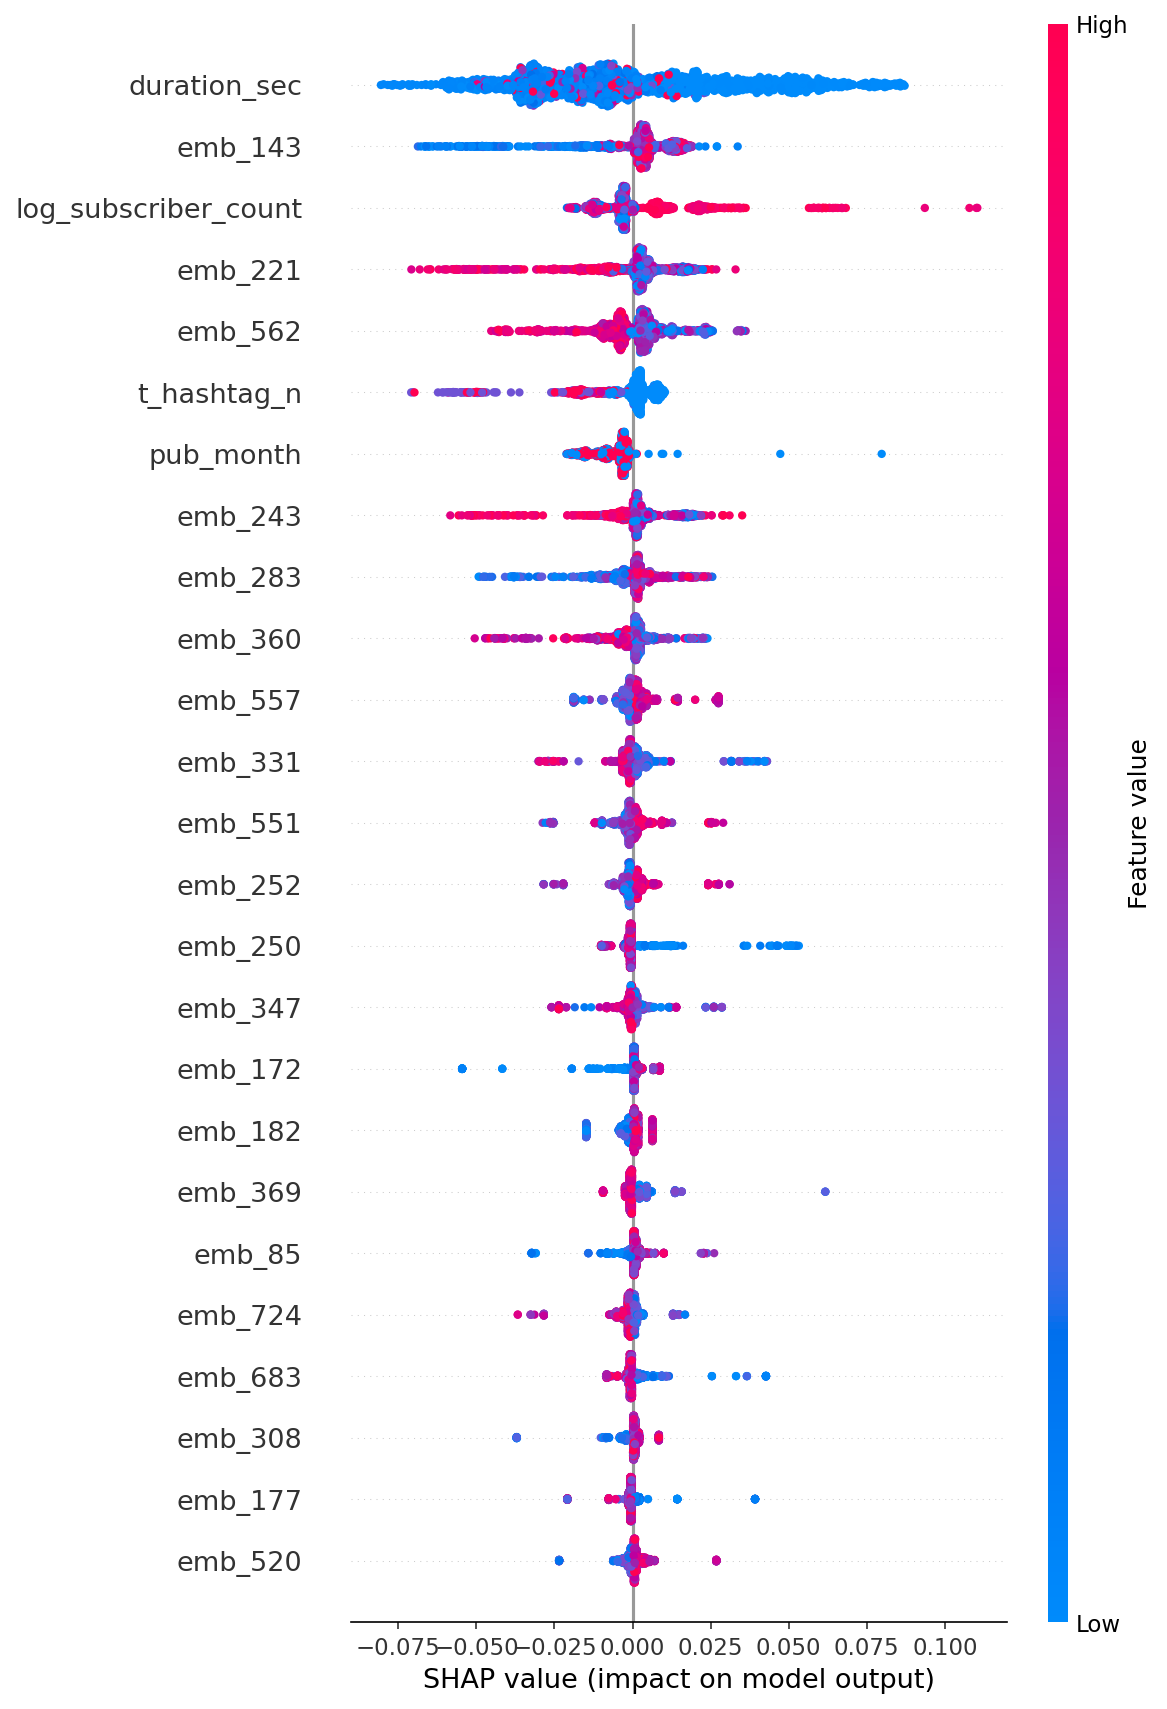
\includegraphics[width=0.85\textwidth]{figures/shap_summary.png}
\caption{SHAP summary plot ของ LightGBM-Structured+TF-IDF จุดสีแดง = ค่า
ฟีเจอร์สูง สีน้ำเงิน = ค่าฟีเจอร์ต่ำ ตำแหน่งแกน $x$ = แรงโน้มน้าวต่อพยากรณ์
ชั้นบวก}
\label{fig:shap}
\end{figure}

\paragraph{การตีความ}
\begin{itemize}[leftmargin=2em]
  \item \texttt{duration\_sec} เป็นฟีเจอร์ที่มีอิทธิพลสูงสุด: วิดีโอที่
        \emph{สั้นเกินไป} (< 60s, ซึ่งคือ YouTube Shorts) มี SHAP บวกแสดงว่า
        เพิ่มโอกาสไวรัล ส่วนวิดีโอ medium-length (5--15 นาที) มี SHAP ใกล้
        ศูนย์
  \item ฟีเจอร์ \texttt{log\_subscriber\_count} ติดอันดับ 3 ยืนยันการค้นพบของ
        \textcite{hoiles2017engagement} ในบริบทไทย
  \item \textbf{มิติของ title embedding หลายตัว} (\texttt{emb\_143},
        \texttt{emb\_221}, \texttt{emb\_562}) ติดอันดับสูง แสดงว่าสัญญาณภาษา
        เชิงลึกจาก SBERT มีคุณค่าเสริมจากฟีเจอร์เชิงโครงสร้างอย่างชัดเจน
        การตีความความหมายของแต่ละ embedding dim ทำได้ยากในเชิงสัญลักษณ์ แต่
        การปรากฏของพวกมันใน top-10 ยืนยันว่า title content ไม่ใช่ noise
  \item \texttt{t\_hashtag\_n} (จำนวน hashtag ในชื่อ) เป็นสัญญาณบวก: วิดีโอที่
        ผู้สร้างใส่ hashtag มักเป็น content ที่ออกแบบเพื่อ discoverability
\end{itemize}

\subsection{LIME บน PhayaThaiBERT}

ตารางที่ \ref{tab:lime-top} แสดง token ที่มี aggregate absolute weight สูง
ที่สุดจาก LIME บน 50 ตัวอย่าง

\begin{table}[H]
\centering
\caption{Top tokens by aggregate $|$LIME weight$|$ on PhayaThaiBERT}
\label{tab:lime-top}
\begin{tabularx}{\textwidth}{lXr}
\toprule
\textbf{Rank} & \textbf{Token} & \textbf{$\sum|w|$} \\
\midrule
1 & \texttt{roblox}                     & 0.251 \\
2 & \texttt{Roblox}                     & 0.230 \\
3 & ค (ส่วนของ ``คน'', ``ความ'')        & 0.177 \\
4 & ``งสารมากคร'' (substring)            & 0.122 \\
5 & ``นในป'' (substring)                & 0.116 \\
6 & น                                    & 0.105 \\
7 & RoV                                  & 0.100 \\
8 & า                                    & 0.091 \\
9 & ``ผมเป'' (จาก ``ผมเป็น'')           & 0.091 \\
10 & ฟอร์เม                              & 0.085 \\
\bottomrule
\end{tabularx}
\end{table}

\paragraph{การตีความ}
ชื่อเกม \texttt{Roblox} และ \texttt{RoV} ปรากฏที่อันดับสูง สะท้อนว่าหมวด
Gaming มีคำเฉพาะที่ขับเคลื่อนความไวรัล ส่วน substring ภาษาไทยที่อยู่ในอันดับ
สูง (ค, น, า) เกิดจากตัวตัดคำ SentencePiece ของ PhayaThaiBERT ที่ตัดคำ
ภาษาไทยเป็น sub-word ขนาดเล็ก

\subsection{Attention Rollout บน PhayaThaiBERT}

ใช้สูตร \eqref{eq:attnroll} กับ PhayaThaiBERT บนตัวอย่าง 20 ชิ้นจากชุดทดสอบ
ความสนใจรวมจาก \texttt{[CLS]} token ไปยัง input tokens แต่ละตัว ถูกบันทึกเป็น
HTML heatmap ต่อตัวอย่างใน \texttt{reports/figures/attention/attention\_html/}
และ aggregate ที่ \texttt{reports/figures/attention/attention\_rollout\_per\_example.parquet}

ผลเชิงคุณภาพคือ ใน 2 ตัวอย่างที่ทำนายถูก attention มักรวมไปที่ token ที่เป็น
\emph{เอนทิตี} (ชื่อเกม, ชื่อบุคคล) หรือ \emph{คำที่มีอิโมจิ} ในตัวอย่างที่
ทำนายผิด attention กระจายตัวอย่างไม่มีจุดเด่นชัด แสดงว่าแบบจำลองขาดสัญญาณที่
discriminative

\subsection{การวิเคราะห์ Top False Positives/Negatives}

จากไฟล์ \texttt{reports/tables/errors\_top\_fp\_stacking\_stacking\_lr\_calibrated.csv}
และ \texttt{errors\_top\_fn\_*.csv} เราพบรูปแบบการผิดพลาดดังนี้

\paragraph{False Positives (พยากรณ์ว่าไวรัล แต่ไม่ไวรัลจริง)}
\begin{itemize}[leftmargin=2em]
  \item วิดีโอจากช่องขนาดใหญ่ที่มี engagement rate ต่ำกว่าค่าเฉลี่ยของช่อง
  \item ชื่อมีคำกระตุ้น clickbait มากแต่เนื้อหาไม่ตรง ทำให้ engagement ลด
  \item โพสต์ในช่วง off-peak (เช้ามืด) เป็นวันธรรมดา
\end{itemize}

\paragraph{False Negatives (พยากรณ์ว่าไม่ไวรัล แต่ไวรัลจริง)}
\begin{itemize}[leftmargin=2em]
  \item วิดีโอจากช่อง mid-size ที่ ``ติด'' โดยไม่คาดคิด มักได้รับการแชร์
        ภายนอกแพลตฟอร์ม (TikTok, X)
  \item ชื่อภาษาไทยล้วน ไม่มีอีโมจิ ไม่มีคำกระตุ้น เป็นความสำเร็จที่อาศัย
        เนื้อหาในวิดีโอเอง
  \item วิดีโอ MV ใหม่ของศิลปินที่กำลังโด่งดัง — สัญญาณนี้อยู่ภายนอก meta-data
\end{itemize}

\subsection{สรุปการวิเคราะห์ความสามารถในการอธิบาย}

จาก SHAP, LIME และ attention rollout เราพบรูปแบบที่สอดคล้องกัน:
\textbf{สัญญาณที่ใช้พยากรณ์ส่วนใหญ่อยู่ในฟีเจอร์เชิงโครงสร้าง} (ขนาดช่อง
ความถี่อัปโหลด ความยาววิดีโอ) ส่วนสัญญาณจากภาษาเสริมผ่านการระบุเอนทิตี
สำคัญในชื่อ (ชื่อเกม ชื่อบุคคล) และการมีอีโมจิ ภาษาไทยที่ละเอียดในระดับ
ความหมายเชิงลึก \emph{ยังไม่ใช่} เกณฑ์ที่ขับเคลื่อนการพยากรณ์ ภายใต้ข้อมูลขนาด
นี้ การรวมแบบจำลองหลายตัวจึงสำคัญ — แต่ละแบบจำลองให้ ``มุม'' ที่แตกต่างกัน
ตามที่ Cochran's Q ยืนยัน

\section{สรุปการตอบสมมติฐาน}
\label{sec:results-summary}

\begin{table}[H]
\centering
\caption{การสรุปการตอบสมมติฐานของการวิจัย}
\label{tab:hypothesis-summary}
\begin{tabularx}{\textwidth}{lXc}
\toprule
\textbf{สมมติฐาน} & \textbf{เนื้อหา} & \textbf{สรุป} \\
\midrule
$H_1$ & PhayaThaiBERT $>$ WangchanBERTa & \textbf{ยืนยัน} (0.6451 vs 0.6402, $p=10^{-7}$) \\
$H_2$ & XLM-R-large $\geq$ monolingual Thai LMs & \textbf{ปฏิเสธ} (0.5450 ต่ำสุด) \\
$H_3$ & Stacking $>$ best single & \textbf{ยืนยัน} (0.6914 vs 0.6728, $p=6.9{\times}10^{-53}$) \\
$H_4$ & รูปแบบความผิดพลาดของ encoders ต่างกัน & \textbf{ยืนยัน} ($p=9{\times}10^{-134}$) \\
\bottomrule
\end{tabularx}
\end{table}

ผลการทดลองยืนยัน 3 ใน 4 สมมติฐาน ส่วน $H_2$ ที่ถูกปฏิเสธให้ข้อมูลเชิงลึกที่
สำคัญ: \textbf{สำหรับงานจำแนกข้อความสั้นภาษาไทยที่มีข้อมูลจำกัด แบบจำลอง
multilingual ขนาดใหญ่ไม่สามารถเอาชนะ monolingual แบบ targeted ได้}
ข้อสรุปนี้สอดคล้องกับงานของ \textcite{lin2022few} ที่พบรูปแบบเดียวกัน
ใน few-shot learning ของภาษา low-resource: ขนาดของแบบจำลองมัลติลิงกัวล
ไม่ได้ทดแทนคลังข้อมูลฝึกล่วงหน้าที่หนาแน่นในภาษาเฉพาะกลุ่ม
